\section{Methods}\label{meth}
% TODO
\begin{figure}[b]
  \begin{subfigure}[b]{.47\textwidth}
    \centering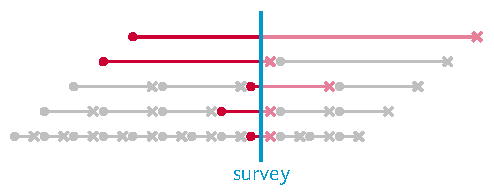
\includegraphics[scale=.75]{diag.group}
    \caption{TODO}
    \label{fig:diag.group}
  \end{subfigure}%
  \begin{subfigure}[b]{.53\textwidth}
    \centering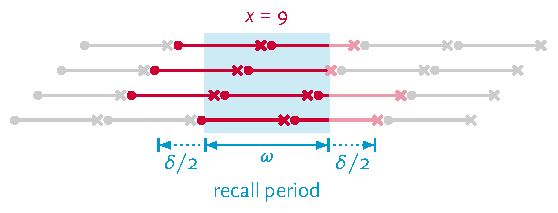
\includegraphics[scale=.75]{diag.partners}
    \caption{TODO}
    \label{fig:diag.partners}
  \end{subfigure}
\end{figure}
%---------------------------------------------------------------------------------------------------
\subsection{Risk Group Duration}\label{meth.yss}
The FSW survey data include questions about
the current respondent's age, and the age of first selling sex.
The difference between these ages could be used to define a ``duration selling sex''.
Using this naive approach, the unadjusted durations $D'_s$ among FSW in Eswatini were
median [IQR] years: 4~[2,~7] in 2011 and 5~[3,~9] in 2014.
However, such estimates have three sources of bias:
sampling error, measurement error, and censoring.
\par
Sampling error was considered via RDS-adjustment in the 2011 survey (only),
yielding estimates of the proportions of FSW
who had sold sex starting 0--2, 3--5, 6--10, and 10+ years ago.
The adjusted proportions indicate fewer years selling sex \vs the unadjusted proportions,
which would be consistent with
challenges in reaching women in the first year(s) of sex work \cite{Cheuk2020}.
Fitting an exponential distribution to the cumulative adjusted proportions
(Appendix~\ref{app.yss})
yielded an estimated distribution mean $\bar{D}_s$ of 4.2 (95\%~CI: 3.5,~5.3) years.
\par
Regarding measurement error: FSW may not sell sex continuously.
The 2014 survey (only) asked whether respondents ever stopped selling sex
and 348/777 (45\%) had stopped at least once.
Among these FSW, the expected duration selling sex in the current period
(\ie since re-starting most recently)
must be less than half ($\rho < 1/2$) of the durations above,
depending on the number and lengths of gaps in selling sex.
Thus, a further adjustment to the mean duration could be defined as:
$(0.45\,\rho + 0.55)\,\bar{D}_s$,
with $\rho \sim \distr{Unif}{0.2,0.4}$ as an assumption.
\par
Finally, these durations are also right censored
because almost all respondents will continue selling sex after the survey \cite{Fazito2012}.
If we assume that the survey reaches FSW
at a random time point during their total (eventual) duration selling sex $D$,
then the duration reported in the survey is effectively $D_s \sim \distr{Unif}{0,D}$.
Thus, the mean duration reported in the survey is $\bar{D}_s = \frac12 \bar{D}$,
and we can define $f = \bar{D} / \bar{D}_s = 2$,
to give the final adjusted estimate as:
$\bar{D} = f\,(0.45\,\rho + 0.55)\,\bar{D}_s$.
In case the RDS-adjustment did not actually account for
delayed self-identification as FSW \cite{Cheuk2020},
we could use $f \sim \distr{Unif}{1.5,2}$.
\par
Figure~\ref{fig:diag.group} illustrates the censoring issue
in a steady-state population with 5 women selling sex at any given time.
Another observation we can make from Figure~\ref{fig:diag.group} is that
women who sell sex longer are more likely to be captured in the survey.
That is, while the sampled durations are representative of women who \emph{currently} sell sex,
these durations are biased high \vs the population of women who \emph{ever} sell sex.
%---------------------------------------------------------------------------------------------------
\subsection{Sexual Partnership Duration}\label{meth.partners}
The FSW surveys asked respondents to report
their numbers of unique sexual partners in the past 30 days,
stratified by three types of partner:
new paying clients, regular paying clients, and non-paying partners.
For illustrative purposes, we assume that
only a small proportion of new clients would go on to become regular clients;
thus, we conceptualize ``new'' clients as effectively ``one-off'' clients.
We further assume that partnership durations were:
1~day with new paying clients,
4~months with regular paying clients, and
3~years with non-paying partners 
(no survey questions asked about partnership durations) \cite{?}.
\par
Using the published aggregate statistics in \cite{Baral2014,EswKP2014},
the reported numbers of partnerships of each type were, respectively:
1.77, 4.69, and 0.74 in 2011 (RDS-adjusted medians), and
5.04, 8.03, and 1.22 in 2014 (unadjusted means).
Our aim is to use these reported numbers of partners ($x$)
for the 30-day recall period ($\omega$),
with the assumed partnership durations ($\delta$),
to define expected rates of partnership change ($Q$) and numbers of concurrent partnerships ($K$).
\par
We begin with some general observations about
the relationships between the variables $x, \omega, \delta, Q, K$.
If partnership duration is long and the recall period is short ($\delta \gg \omega$),
the reported partnerships mostly reflect \emph{ongoing} partnerships,
and thus $x \approx K$.
If partnership duration is short and the recall period is long ($\delta \ll \omega$),
the reported partnerships mostly reflect \emph{complete} partnerships,
and thus $x/\omega \approx Q$.
However, if partnership duration and recall period are similar in length,
the reported partnerships reflect a mixture of tail-ends, complete, and ongoing partnerships,
and thus $x$ overestimates $K$, but $x/\omega$ also overestimates $Q$.
\par
Next, we make a similar assumption as in \sref{meth.yss}:
that survey timing is effectively random with respect to partnership duration.
Then, if either end of the recall period would capture an ongoing partnership,
the intersection point would be, on average, at the partnership mid-point.
Thus, the recall period is effectively extended
by half the partnership duration $\delta/2$ on each end, and $\delta$ overall,
as illustrated in Figure~\ref{fig:diag.partners}.
As such, we can define $Q$ and $K$ as:
\begin{alignat}{1}
  Q &= \frac{x}{\omega + \delta}\\
  K &= \frac{x \delta}{\omega + \delta} = Q \delta
\end{alignat}
\par
As an example, Figure~\ref{fig:diag.partners} also illustrates
a recall period of $\omega = 1$ year,
for which $x = 9$ partnerships are reported,
having durations of $\delta = 0.75$ years.
Thus, we can compute
$Q = 9/(1+0.75) = 5.14$ partnerships per year and
$K = 5.14(0.75) = 3.86$ current partners;
these ars slight underestimates of the true values $Q = 5.33, K = 4$,
due to randomness in the exact ``location'' of the recall period.
